\documentclass[conference]{IEEEtran}
\usepackage{graphicx,booktabs,amsmath,amssymb,hyperref,xcolor,tikz,array,multirow}
\usetikzlibrary{arrows.meta,positioning,fit,calc}
\hypersetup{colorlinks=true,linkcolor=blue!50!black,citecolor=blue!50!black,urlcolor=blue!50!black}

% placeholder macro: anything still to be measured is shown in red brackets
\newcommand{\tbd}[1]{\textcolor{red}{[\textbf{TBD:} #1]}}
\newcommand{\hyp}[1]{\textbf{#1}}

\begin{document}

\title{Perception-Guided Reinforcement Learning for Ballbot Navigation\\on Uneven Terrain in Simulation}
\author{\IEEEauthorblockN{Nebiyu Tadesse}
\IEEEauthorblockA{Johns Hopkins University\\
Course: Artificial Intelligence for Robotics (draft for instructor review)}}
\maketitle

\begin{abstract}
A ballbot is an underactuated robot that balances on a single ball and moves by controlled leaning. Navigating uneven terrain requires the robot to keep its balance and make progress at the same time, using only limited sensing. We study this problem in simulation, starting from the open-source MuJoCo benchmark and PPO pipeline of Salehi (2025). Our first result is diagnostic: the pipeline as released does not train on a stock MuJoCo installation. We identify three causes: (i) the omniwheel anisotropic friction relies on a collision-frame patch to MuJoCo, and on stock MuJoCo two of the three wheels get the wrong friction direction; (ii) the velocity used by the directional reward was read from the wrong half of MuJoCo's 6-D velocity vector, so the reward paid for angular rather than linear velocity; and (iii) the default Perlin terrain is far steeper (mean slope $\approx 46^\circ$) than the $20^\circ$ tilt limit. We repair all three in software, re-tune PPO, and train proprioception-only and proprioception$+$depth policies. We evaluate on held-out terrain seeds and difficulties and test three hypotheses: \hyp{H1} adding depth improves success and reduces falls; \hyp{H2} performance degrades under depth noise and occlusion; \hyp{H3} a goal signal improves time-to-goal over open-loop directional drive. In our preliminary results (two seeds per variant, 1M decisions), depth did not reduce falls (H1 not supported) and corrupting or even blanking the depth input changed nothing (the policies ignore it, so the H2 drop is not observed); the waypoint stretch (H3) is inconclusive.. The full code, configs, and notebook are included.
\end{abstract}

\begin{IEEEkeywords}
ballbot, reinforcement learning, PPO, depth perception, rough-terrain navigation, MuJoCo
\end{IEEEkeywords}

%=====================================================================
\section{Introduction}
%=====================================================================
A ballbot is a tall, narrow robot that balances dynamically on a single sphere driven by actuated rollers or omniwheels \cite{lauwers2006,nagarajan2014}. Because its support polygon collapses to one contact point, it is omnidirectional and agile, and it is statically unstable: if the controller stops, the robot falls. Classical ballbot control derives Lagrangian dynamics and stabilises decoupled planar models with PID/LQR-style controllers on a flat floor \cite{nagarajan2014,abdelrahim2025}. These assumptions (flat ground, no slip between ball and floor) are exactly what is violated when the robot must \emph{navigate} over uneven ground.

\textbf{Task.} We consider goal-directed navigation of a simulated ballbot on procedurally generated uneven terrain. At every decision step the policy outputs normalised commands for three omniwheel motors. The episode succeeds if the robot makes a required amount of progress along a target direction without exceeding a $20^\circ$ tilt (a fall).

\textbf{Environment and sensing.} The robot is simulated in MuJoCo \cite{todorov2012} at 500\,Hz. It senses (i) proprioception: orientation, angular and linear velocity, wheel speeds and the previous action; and (ii) two low-resolution depth cameras ($64{\times}64$) aimed at the ball--ground contact region, which reveal terrain the proprioceptive state alone cannot disambiguate \cite{salehi2025}.

\textbf{Goals.} (1) Reproduce a working baseline of \cite{salehi2025,salehi2025code}; (2) study how perception and goal specification affect navigation (proprioception-only vs.\ proprioception$+$depth; depth noise and occlusion; an optional waypoint signal); (3) report clear metrics (success, fall rate, return, time-to-goal and robustness) on held-out terrain seeds and difficulties.

\textbf{Contributions.} (i) A root-cause analysis of why the baseline does not train on a stock simulator, including a velocity-indexing bug in the reward (Sec.~\ref{sec:method-physics}); (ii) software fixes that make it train; (iii) a controlled comparison of perception variants with paired statistics on held-out terrains; (iv) an open, runnable notebook and scripts.

%=====================================================================
\section{Related Work}
%=====================================================================
\textbf{Ballbot dynamics and control.} Lauwers et al.\ built the first practical ballbot with an inverse mouse-ball drive \cite{lauwers2006}. Nagarajan et al.\ derived the Lagrangian dynamics and demonstrated decoupled planar balancing and trajectory control on a human-sized ballbot with an omniwheel drive \cite{nagarajan2014}; their controllers assume a flat, level floor and linearised dynamics. Subsequent work covers drivetrain design for agility and payload \cite{xiao2023}, systematic modelling and control \cite{abdelrahim2025}, and motion planning among people with topology-informed MPC \cite{mavrogiannis2021}. Carius et al.\ control a simulated ballbot on uneven ground with a path-integral stochastic optimal control method whose rollouts come from a physics engine \cite{carius2022}.

\textbf{Learning for ballbots.} Zhou et al.\ cast balancing as a recovery task and combine a conventional feedback controller with deep RL in a compound controller that tolerates larger initial tilts \cite{zhou2022}. Salehi (2025) was the first to learn \emph{navigation} on random uneven terrain with model-free RL: a PPO policy \cite{schulman2017} conditioned on proprioception and on features of two depth images produced by a pretrained, frozen autoencoder encoder \cite{salehi2025}. It also released the MuJoCo simulator and training code \cite{salehi2025code}.

\textbf{Learning-based rough-terrain locomotion.} In legged robots, policies trained in simulation with RL transfer to hardware \cite{hwangbo2019}; proprioception alone can already traverse challenging terrain \cite{lee2020}, and fusing exteroception with proprioception improves robustness, including when perception is noisy or missing \cite{miki2022}. Massively parallel PPO with terrain curricula makes such training fast \cite{rudin2022}. Our H1/H2 transfer these perception questions to the ballbot, where the base is far less stable than a legged robot.

\textbf{Position relative to Salehi (2025).} We use the same simulator family, observation structure, depth encoder and PPO method. We differ in three ways: (1) we expose and fix three reproducibility problems (friction frame, velocity indexing in the reward, terrain steepness) and re-tune the learning setup; (2) we add the controlled ablations absent from the original: proprioception-only vs.\ depth, and perception corruption; (3) we report success/fall metrics with paired statistics on disjoint held-out terrains rather than only learning curves.

%=====================================================================
\section{Research Problem and Hypotheses}
%=====================================================================
We model navigation as an MDP $\langle \mathcal{S},\mathcal{A},P,P_0,R,\gamma\rangle$ \cite{schulman2017}. The policy $\pi_\theta(a_t\mid o_t)$ maps an observation $o_t$ to $a_t\in[-1,1]^3$. The terrain is sampled from a Perlin-noise distribution \cite{perlin1985} with difficulty (amplitude) $A$ and seed $\sigma$; $A$ controls slope. Training uses seeds $\sigma<10^4$ and $A\sim U(0.02,0.14)$; testing uses disjoint seeds $\sigma\ge 10^5$ at fixed amplitudes, including a harder level outside the training range.

\textbf{Observation ambiguity.} With proprioception only, two situations with identical $(\zeta,\dot\zeta,v,\dot m,a_{t-1})$ may face different terrain ahead; depth is the only channel that can resolve this \cite{salehi2025}.

\textbf{Metrics.} Per held-out episode we record: \emph{success} (reaches $d^\ast$ m of progress along the target direction $g$ without falling within $T$ steps), \emph{fall} (tilt $>20^\circ$), \emph{return}, \emph{time-to-goal} (first step reaching $d^\ast$), and mean speed. Progress is $p_t=\langle \mathbf{x}_t - \mathbf{x}_0, g\rangle$.

\begin{itemize}
\item[\hyp{H1}] PPO with proprioception$+$depth achieves higher success and lower fall rate on held-out terrains than proprioception-only.
\item[\hyp{H2}] Success degrades under depth noise and partial occlusion; the drop quantifies reliance on vision.
\item[\hyp{H3}] (stretch) A simple goal/waypoint signal reduces time-to-goal relative to open-loop directional drive on the same terrains.
\end{itemize}
Statistical plan: paired comparisons over identical terrains (same seed and amplitude), reporting the mean difference with a bootstrap 95\% CI and a Wilcoxon signed-rank $p$-value, and Wilson intervals for rates; training seeds are treated as replicates \cite{henderson2018,agarwal2021}.

%=====================================================================
\section{Method}
%=====================================================================
\subsection{Sensing $\rightarrow$ decision $\rightarrow$ action}
Fig.~\ref{fig:block} shows the pipeline. Proprioception $o^{\text{prop}}_t\in\mathbb{R}^{15}$ is z-scored with running statistics. Each depth image $I^{(c)}_t\in[0,1]^{64\times64}$ ($c\in\{0,1\}$) is mapped by a convolutional encoder $E$ (two stride-2 $3{\times}3$ conv layers with batch norm and LeakyReLU, then a linear layer to 20 units with $\tanh$) to $z^{(c)}_t\in\mathbb{R}^{20}$. The concatenation $[o^{\text{prop}}_t, z^{(0)}_t, z^{(1)}_t]\in\mathbb{R}^{55}$ feeds actor and critic MLPs ($2{\times}256$, $\tanh$). The encoder is the autoencoder encoder released with \cite{salehi2025}, \emph{frozen} and kept in evaluation mode (fixed batch-norm statistics); the variant without cameras has a 15-dimensional input and renders no images.

\begin{figure*}[t]
\centering
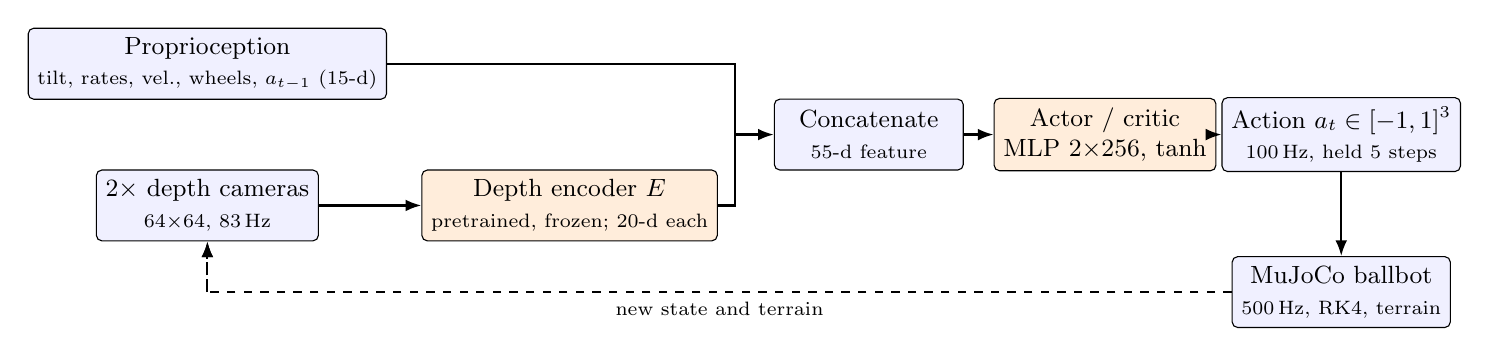
\begin{tikzpicture}[font=\small,
  box/.style={draw, rounded corners=2pt, minimum height=9mm, minimum width=24mm, align=center, fill=blue!6},
  pbox/.style={draw, rounded corners=2pt, minimum height=9mm, minimum width=24mm, align=center, fill=orange!14},
  arr/.style={-{Latex[length=2mm]}, thick}]
 \node[box] (imu) at (0,0.9) {Proprioception\\{\scriptsize tilt, rates, vel., wheels, $a_{t-1}$ (15-d)}};
 \node[box] (cam) at (0,-0.9) {2$\times$ depth cameras\\{\scriptsize $64{\times}64$, 83\,Hz}};
 \node[pbox] (enc) at (4.6,-0.9) {Depth encoder $E$\\{\scriptsize pretrained, frozen; 20-d each}};
 \node[box] (cat) at (8.4,0) {Concatenate\\{\scriptsize 55-d feature}};
 \node[pbox] (mlp) at (11.4,0) {Actor / critic\\MLP $2{\times}256$, tanh};
 \node[box] (act) at (14.4,0) {Action $a_t\in[-1,1]^3$\\{\scriptsize 100\,Hz, held 5 steps}};
 \node[box] (sim) at (14.4,-2.0) {MuJoCo ballbot\\{\scriptsize 500\,Hz, RK4, terrain}};
 \coordinate (join) at (6.7,0);
 \draw[arr] (cam) -- (enc);
 \draw[thick] (imu.east) -| (join);
 \draw[thick] (enc.east) -| (join);
 \draw[arr] (join) -- (cat.west);
 \draw[arr] (cat) -- (mlp);
 \draw[arr] (mlp) -- (act);
 \draw[arr] (act) -- (sim);
 \draw[arr, dashed] (sim.west) -- (0,-2.0) node[midway, below]{\scriptsize new state and terrain} -- (cam.south);
 \draw[arr, dashed] (0,-2.0) -- (cam.south);
\end{tikzpicture}
\caption{Sensing$\rightarrow$decision$\rightarrow$action flow. Orange blocks are learned or pretrained networks; the proprioception-only variant omits the cameras and the encoder.}
\label{fig:block}
\end{figure*}


\begin{figure*}[t]
\centering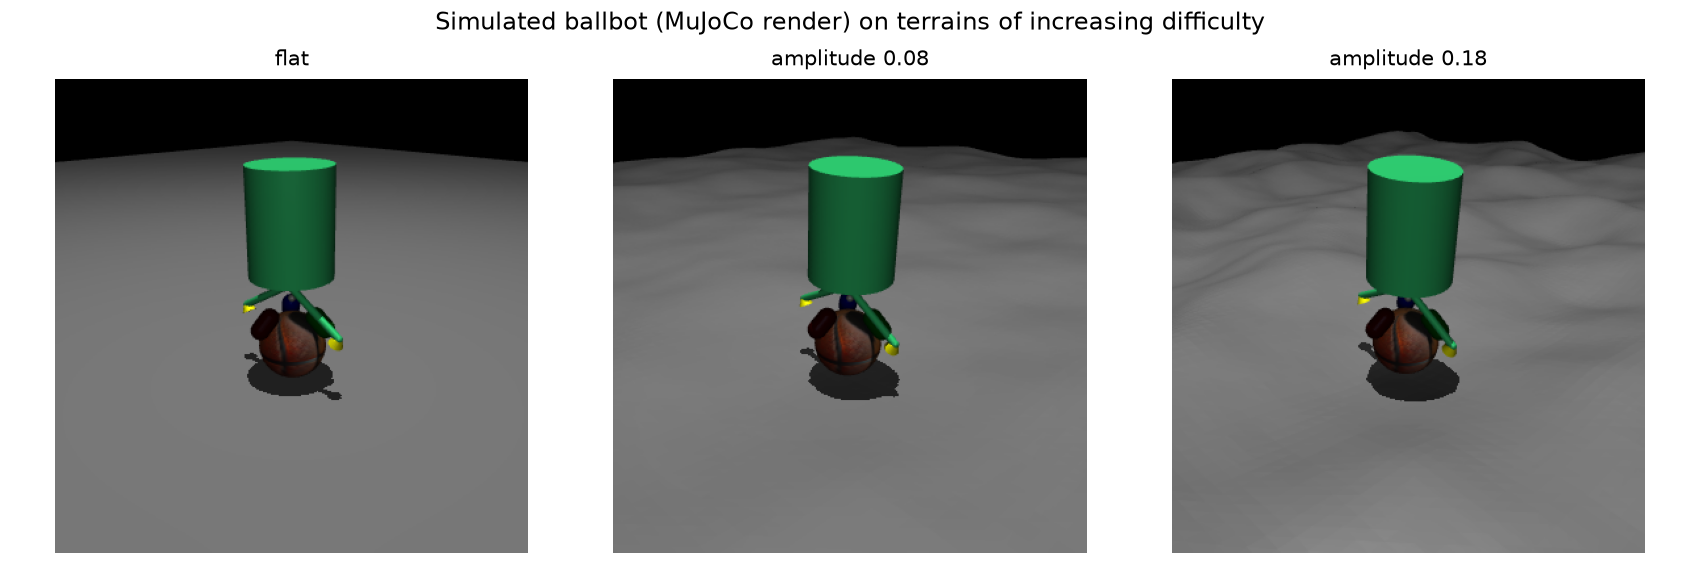
\includegraphics[width=0.9\textwidth]{figures/fig_robot_views.png}
\caption{MuJoCo renders of the simulated ballbot (third-person tracking camera, generated by \texttt{scripts/study/make\_figures.py}) on flat ground and on Perlin terrain of amplitude 0.08 and 0.18.}\label{fig:robot}
\end{figure*}

\begin{figure*}[t]
\centering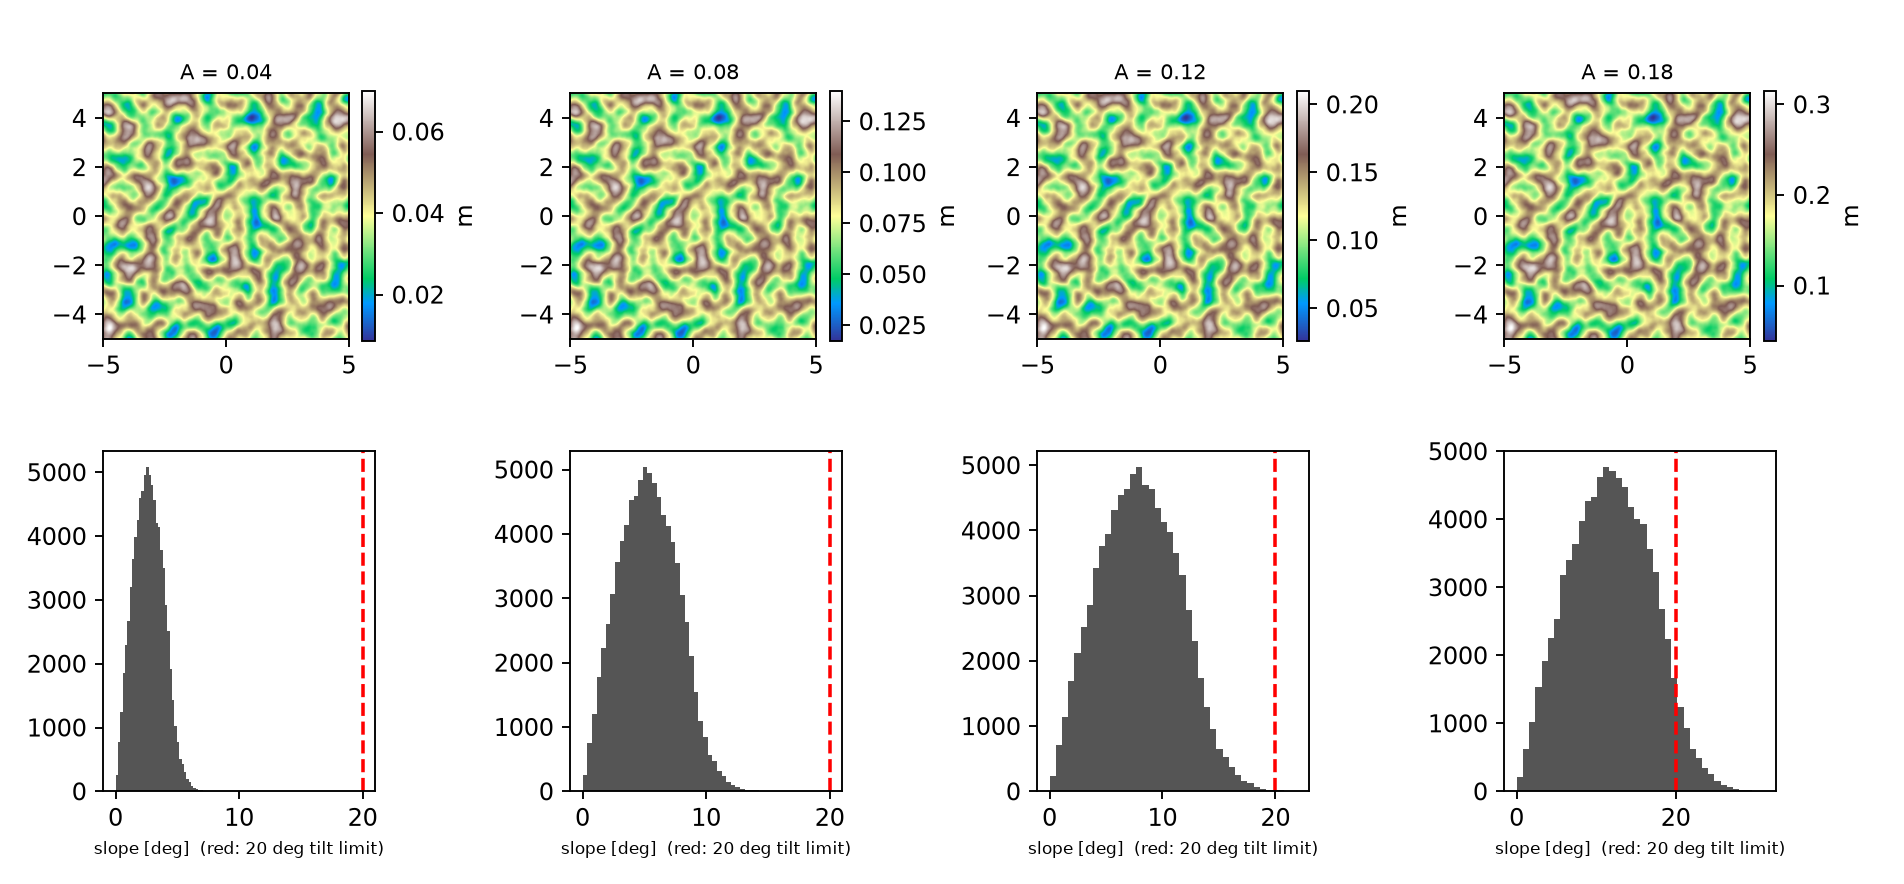
\includegraphics[width=0.85\textwidth]{figures/fig_terrain_levels.png}
\caption{Terrain difficulty: height maps (top) and slope histograms (bottom) for four amplitudes; the red line is the $20^\circ$ tilt limit.}\label{fig:levels}
\end{figure*}

\subsection{Actuation, reward and PPO}
The action is three normalised motor commands scaled by 10 (torque-controlled omniwheels). The policy acts at $100$\,Hz: each action is held for 5 physics steps (2\,ms, RK4). The per-decision reward is
\begin{equation}
r_t = c\,\big(\alpha_1\min(\langle v^{xy}_t,g\rangle,v_{\max}) + \alpha_2\|a_t\|^2 + \alpha_3\,\mathbf{1}[\text{upright}]\big),
\end{equation}
with $c{=}5$ (the action-repeat factor, which keeps returns comparable across control rates), $\alpha_1{=}0.1$ (the baseline uses $0.01$ at 500\,Hz), $\alpha_2{=}-10^{-4}$, $\alpha_3{=}0.02$ and a speed cap $v_{\max}{=}0.6$\,m/s that removes any incentive to lunge forward and fall. Episodes end on a fall (terminal), at an 800-step (8\,s) time limit (truncation, value bootstrapped) or when the goal progress $d^\ast{=}2$\,m is reached (success, truncation).

We optimise with PPO \cite{schulman2017} from Stable-Baselines3 \cite{raffin2021}, GAE($\lambda{=}0.95$) \cite{schulman2016} and the settings in Table~\ref{tab:hp}.

\begin{table}[t]
\centering\caption{PPO setup (ours) versus the released baseline config.}\label{tab:hp}
\small
\begin{tabular}{lcc}
\toprule
 & Baseline \cite{salehi2025code} & Ours \\
\midrule
Control rate & 500\,Hz & 100\,Hz \\
Net (actor/critic) & $4{\times}128$ LeakyReLU & $2{\times}256$ tanh \\
Learning rate & custom schedule & $3\!\cdot\!10^{-4}\!\to\!3\!\cdot\!10^{-5}$ lin. \\
Clip $\epsilon$ & 0.015 & 0.2 \\
$\gamma$ / $\lambda$ & 0.99 / 0.95 & 0.995 / 0.95 \\
Rollout & $10{\times}2048$ & $20{\times}256$ \\
Epochs / batch & 5 / 256 & 8 / 1280 \\
Initial $\log\sigma$ & 0 & $-1$ \\
Normalisation & none & obs (proprio) + reward \\
Target KL & 0.3 & 0.03 \\
\bottomrule
\end{tabular}
\end{table}

\subsection{Making the simulator trainable}\label{sec:method-physics}
\textbf{(1) Omniwheel friction frame.} Each wheel is a capsule with anisotropic ball--wheel friction (\texttt{friction="0.001 1.0"}), which only models an omniwheel if the first contact tangent is the capsule axis. Stock MuJoCo does not guarantee this; the baseline therefore requires a source patch to MuJoCo \cite{salehi2025code}. We measured $|\langle \text{axis}, t_1\rangle|$ on an unpatched MuJoCo 3.13 and found $0.999, 0.209, 0.537$ for the three wheels: only one is aligned. Because building MuJoCo from source was not possible on our machine, we re-implemented the patch in Python: \texttt{ContactFrameStepper} runs RK4 stage by stage and rewrites the wheel-contact frames between collision detection and constraint assembly. With the fix off it matches \texttt{mj\_step} exactly (max difference $0$ over 1000 steps, unit-tested); with it on, all three wheels give $|\langle \text{axis}, t_1\rangle|=1$.

\textbf{(2) Velocity indexing.} MuJoCo's \texttt{cvel} is ordered (rotational, translational). The environment read the \emph{first} three entries as linear velocity, so the observation named ``vel'' was the angular velocity and the directional reward $\langle v^{xy},g\rangle$ rewarded rotation about the horizontal axes. We verified against finite differences of the base position that the \emph{last} three entries are the linear velocity, and swapped them. With the bug, a policy that learned to balance on flat ground made no progress (net displacement $-0.016$\,m in 8\,s); after the fix the same setup moves $1.24$\,m in 8\,s after only 0.3M decisions (Sec.~\ref{sec:exp}).

\textbf{(3) Terrain difficulty.} The default Perlin height field (2\,m vertical scale, amplitude 1) has mean slope $46^\circ$ and 95th percentile $64^\circ$, far above the $20^\circ$ tilt limit. We add an amplitude parameter; amplitudes $0.04, 0.08, 0.12, 0.18$ give mean slopes of roughly $3^\circ$--$13^\circ$ (95th percentile up to $22^\circ$ at $0.2$). A portable NumPy gradient-noise fallback replaces the C \texttt{noise} package, which has no Windows build; it changes the exact noise but not its statistics.

\subsection{Training and evaluation protocol}
Each run uses 20 parallel environments, one random seed, and 1M decisions (about 2.8 simulated hours at 100\,Hz); two seeds per variant. Variants: \texttt{proprio}, \texttt{depth\_frozen} (\texttt{depth\_e2e}, a CNN trained jointly with PPO, is implemented but not yet evaluated). Evaluation uses the deterministic policy on held-out seeds $\sigma=10^5+7i$ at four amplitudes, 30 episodes per cell (20 for H2). H2 corrupts the depth channel at test time only: additive Gaussian noise ($\sigma_n\in\{0.05,0.15,0.30\}$ in normalised depth), random pixel dropout (20\%), and a square occluder covering 25\% or 50\% of each image.

%=====================================================================
\section{Experiments}\label{sec:exp}
%=====================================================================
\textbf{Status.} All numbers below are measured but preliminary (two seeds, 1M decisions); the draft lists what remains in Sec.~\ref{sec:concl}.

\subsection{Reproduction diagnostics (done)}
Four measurements explain why the earlier replication attempt on this codebase (best return 9.20 and 378-step episodes after 10M steps on flat ground, versus $\approx$86 and 4000 steps reported by Salehi \cite{salehi2025}) did not converge. They were obtained with stock MuJoCo 3.13, the configuration used for all experiments below.

\textbf{(1) Wheel friction frames.} Table~\ref{tab:frame} lists the alignment between each wheel's capsule axis and the first contact tangent $t_1$; only wheel~0 is correct on stock MuJoCo.

\begin{table}[h]
\centering\caption{$|\langle \text{capsule axis},t_1\rangle|$ for the ball--wheel contacts (1 = correctly aligned).}\label{tab:frame}
\small\begin{tabular}{lccc}\toprule
 & Wheel 0 & Wheel 1 & Wheel 2\\ \midrule
Stock MuJoCo 3.13 & 0.999 & 0.209 & 0.537\\
With our frame fix & 1.000 & 1.000 & 1.000\\ \bottomrule
\end{tabular}\end{table}

\textbf{(2) Velocity indexing.} Comparing MuJoCo's \texttt{cvel} with finite differences of the base position, the last three entries are the linear velocity (e.g.\ $(0.017,-0.005)$ vs.\ $(0.016,-0.005)$\,m/s) while the first three are the angular velocity. The environment used the first three as ``velocity''.

\textbf{(3) Terrain steepness.} Table~\ref{tab:slope} gives the slope statistics of the height field (20 held-out seeds per row). The default amplitude of 1 produces slopes that no policy with a $20^\circ$ tilt limit can climb; the amplitudes used in our experiments span $1^\circ$--$12^\circ$ mean slope.

\begin{table}[h]
\centering\caption{Perlin terrain slope versus amplitude $A$ (degrees).}\label{tab:slope}
\small\begin{tabular}{rccc}\toprule
$A$ & mean slope & 95th pct. & max\\ \midrule
0.02 & 1.3 & 2.3 & 3.7\\
0.04 & 2.7 & 4.7 & 7.3\\
0.08 & 5.3 & 9.3 & 14.4\\
0.12 & 7.9 & 13.8 & 21.1\\
0.14 & 9.2 & 15.9 & 24.2\\
0.18 & 11.8 & 20.2 & 30.0\\
1.00 (default) & 46.2 & 63.9 & 72.7\\ \bottomrule
\end{tabular}\end{table}

\textbf{(4) Effect of the fixes on flat ground.} Table~\ref{tab:abl} shows what each repair changes on flat ground with identical PPO settings (proprioception only, 0.3M decisions, deterministic evaluation episode of 8\,s). The released-code row is the best prior replication (10M physics steps at 500\,Hz). Removing the friction fix leaves the robot unable to balance (it falls after 0.36\,s), whereas with the fix the policy balances for the whole episode. The velocity bug did not prevent balancing but removed any drive to move: the policy stood still (net displacement $-0.016$\,m), while the corrected reward gave $1.24$\,m in the same time and budget (an earlier, otherwise identical configuration without the fall penalty).

\begin{table*}[t]
\centering\caption{Effect of the repairs on flat ground (single seed).}\label{tab:abl}
\scriptsize\begin{tabular}{lccc}\toprule
Setup & Steps survived (of 800) & Fell & Net progress [m]\\ \midrule
Prior replication (released code)$^\dagger$ & 378 of 4000 (train mean) & yes & --\\
Stock friction frames, velocity fixed & 36 & yes & 0.00\\
Friction fix, velocity bug (swapped \texttt{cvel}) & 800 & no & $-0.02$\\
Friction fix, velocity fixed (all repairs) & 800 & no & 0.27--1.24$^\ddagger$\\ \bottomrule
\end{tabular}\\[2pt]
{\scriptsize $^\dagger$ training-time mean episode length at 500\,Hz. $^\ddagger$ 1.24\,m without the fall penalty and $\gamma{=}0.995$ at 0.3M decisions; 0.27\,m with the final setting ($\gamma{=}0.999$, fall penalty 10) at the same budget, which trades early speed for stability.}
\end{table*}



\subsection{Qualitative behaviour (MuJoCo renders)}
Fig.~\ref{fig:strip} shows one held-out episode: the scene and the two depth inputs over time. Both cameras are aimed at the ball--ground contact, so much of each image is the ball itself and the visible terrain is a thin strip; this is consistent with the weak use of depth found in H1/H2. Fig.~\ref{fig:traj} overlays top-down trajectories of the two policies on the terrain height map, and Fig.~\ref{fig:tilt} the corresponding tilt angles against the $20^\circ$ fall threshold.

\begin{figure*}[t]
\centering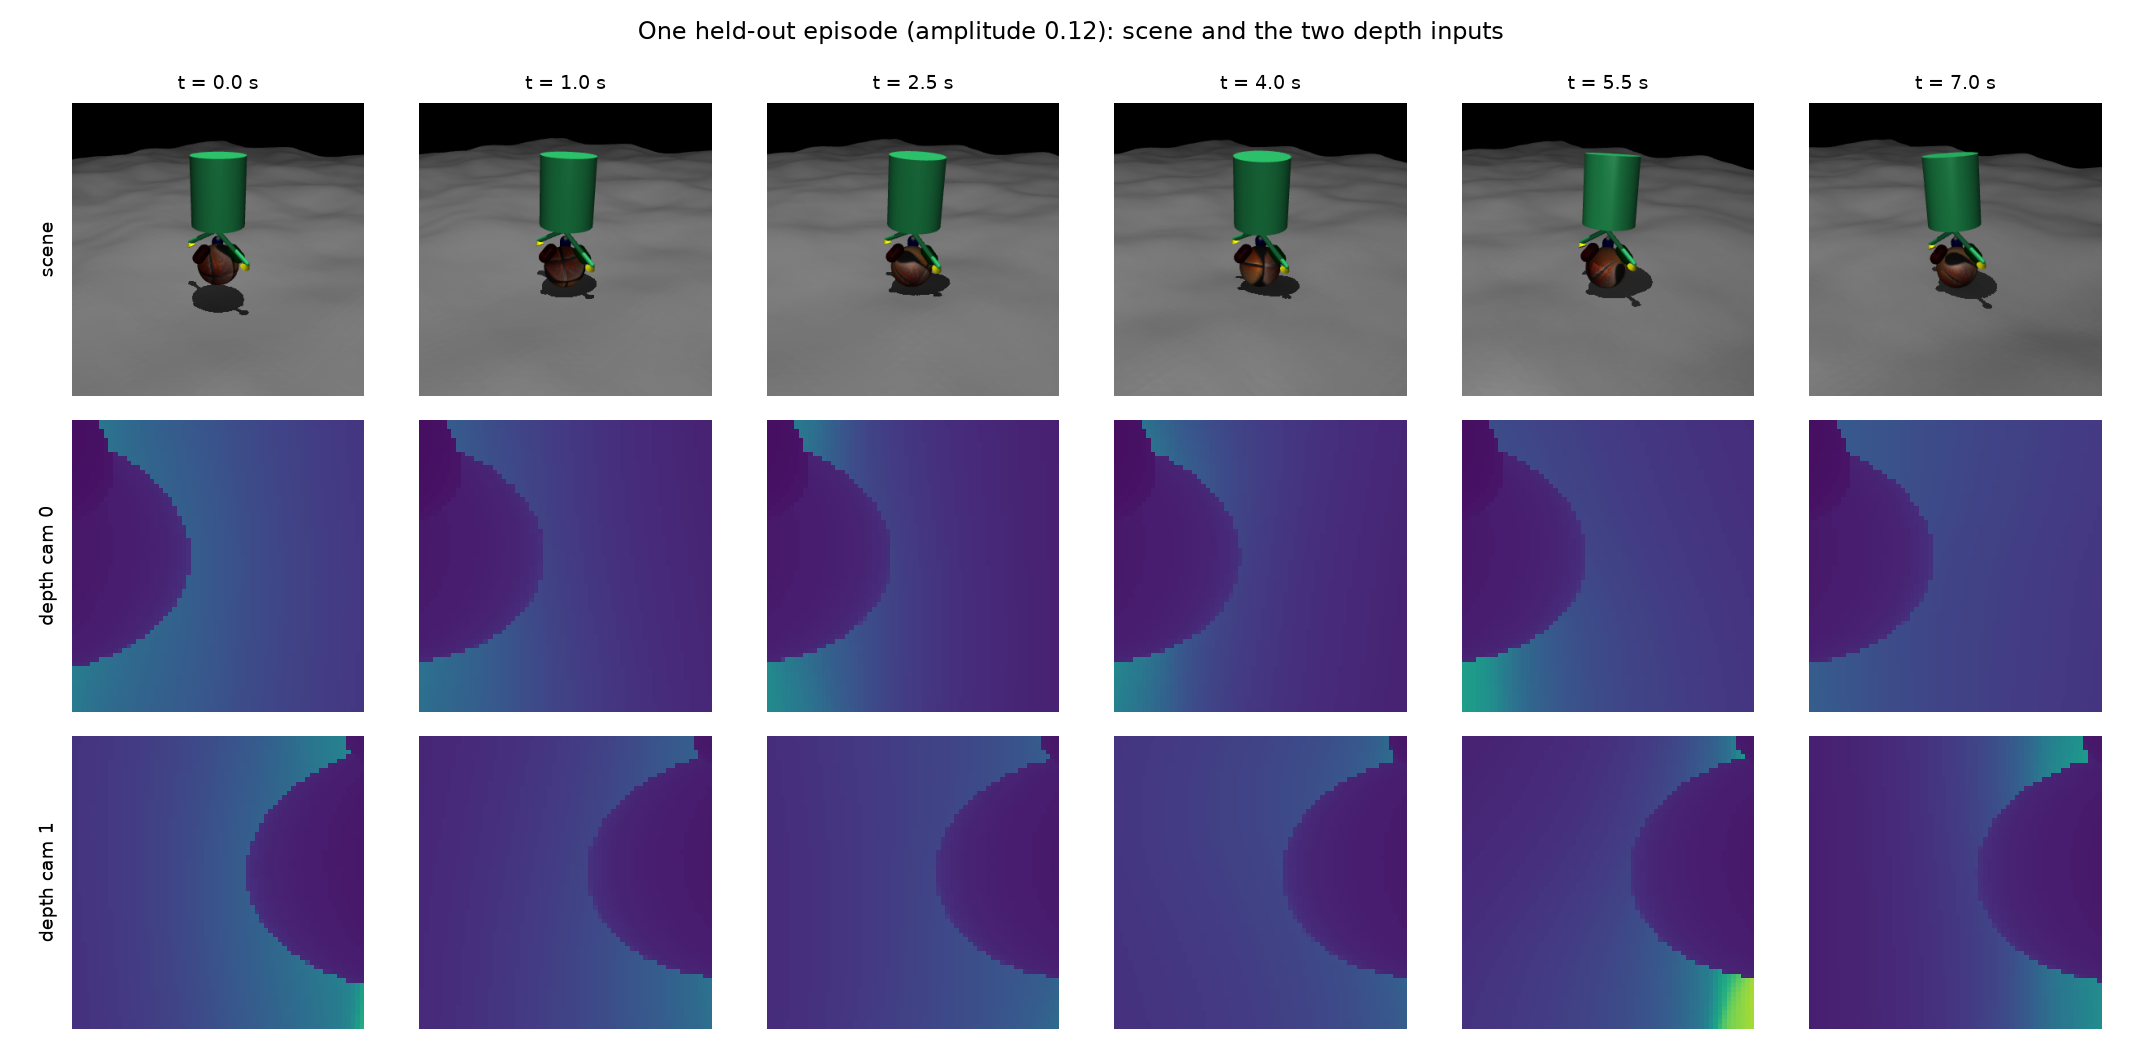
\includegraphics[width=0.95\textwidth]{figures/fig_episode_strip.png}
\caption{Filmstrip of a held-out episode (amplitude 0.12, proprio$+$depth policy): third-person MuJoCo view and the two $64{\times}64$ depth images at six times.}\label{fig:strip}
\end{figure*}

\begin{figure*}[t]
\centering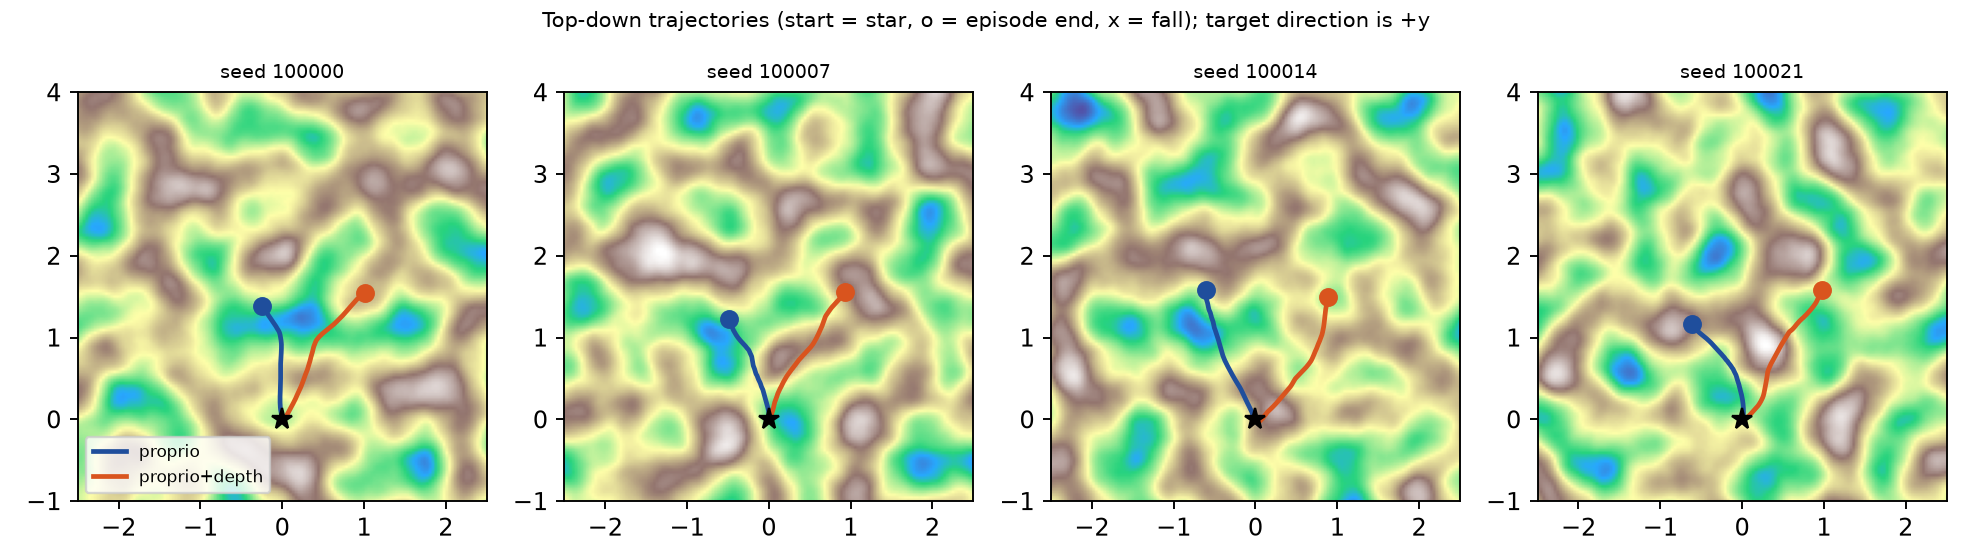
\includegraphics[width=0.95\textwidth]{figures/fig_trajectories.png}
\caption{Top-down trajectories on four held-out terrains (amplitude 0.12) for the proprio-only and proprio$+$depth policies.}\label{fig:traj}
\end{figure*}

\begin{figure*}[t]
\centering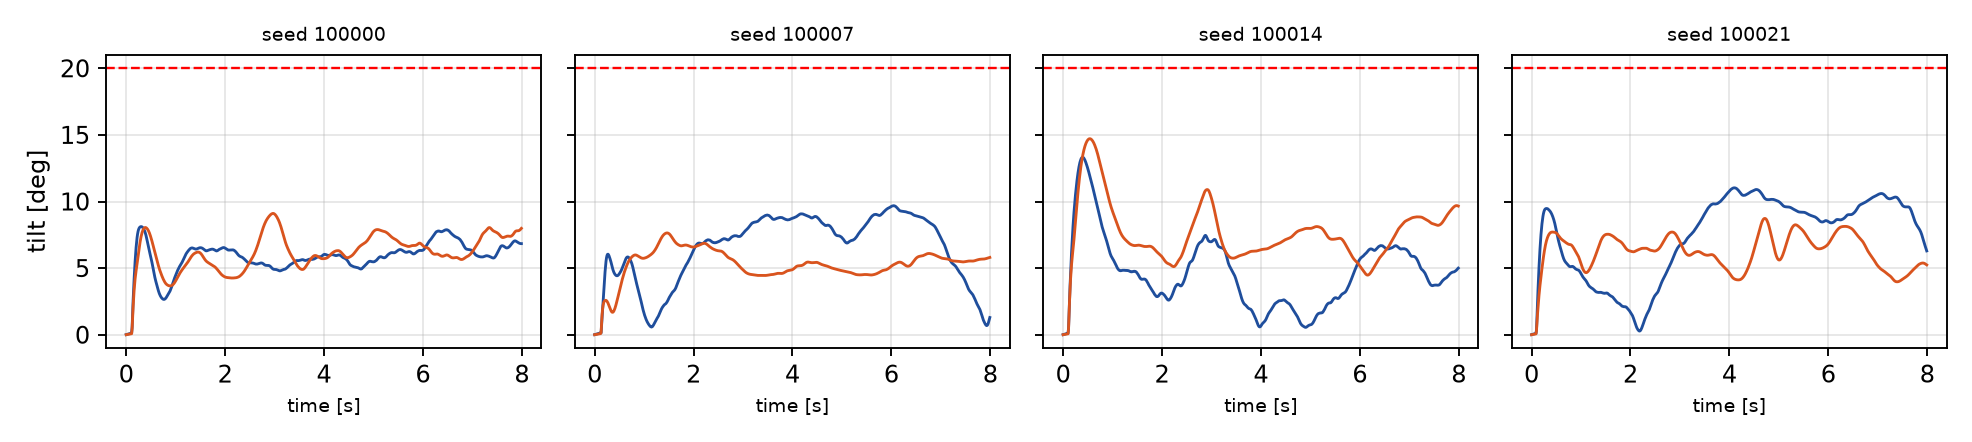
\includegraphics[width=0.95\textwidth]{figures/fig_tilt_time.png}
\caption{Tilt angle over time for the same episodes (blue: proprio, orange: proprio$+$depth; dashed: $20^\circ$ limit).}\label{fig:tilt}
\end{figure*}

\subsection{H1: proprioception vs.\ proprioception$+$depth}
\textbf{Setup.} Two training seeds per variant, 1M decisions each (about 2.8 simulated hours at 100\,Hz), trained on seeds $<10^4$ with $A\sim U(0.02,0.14)$. Evaluation: 30 held-out terrains (seeds $\ge 10^5$) at each of four amplitudes per policy, deterministic actions, 8\,s episodes. Because the policies learned slow, careful driving (0.12--0.22\,m/s, comparable to the $\approx$0.15\,m/s implied by the baseline's reported return), \emph{success} is defined as reaching 1\,m of progress along the target direction without a fall. Fig.~\ref{fig:train} shows the learning curves and Table~\ref{tab:h1} the held-out results.

\begin{figure}[t]
\centering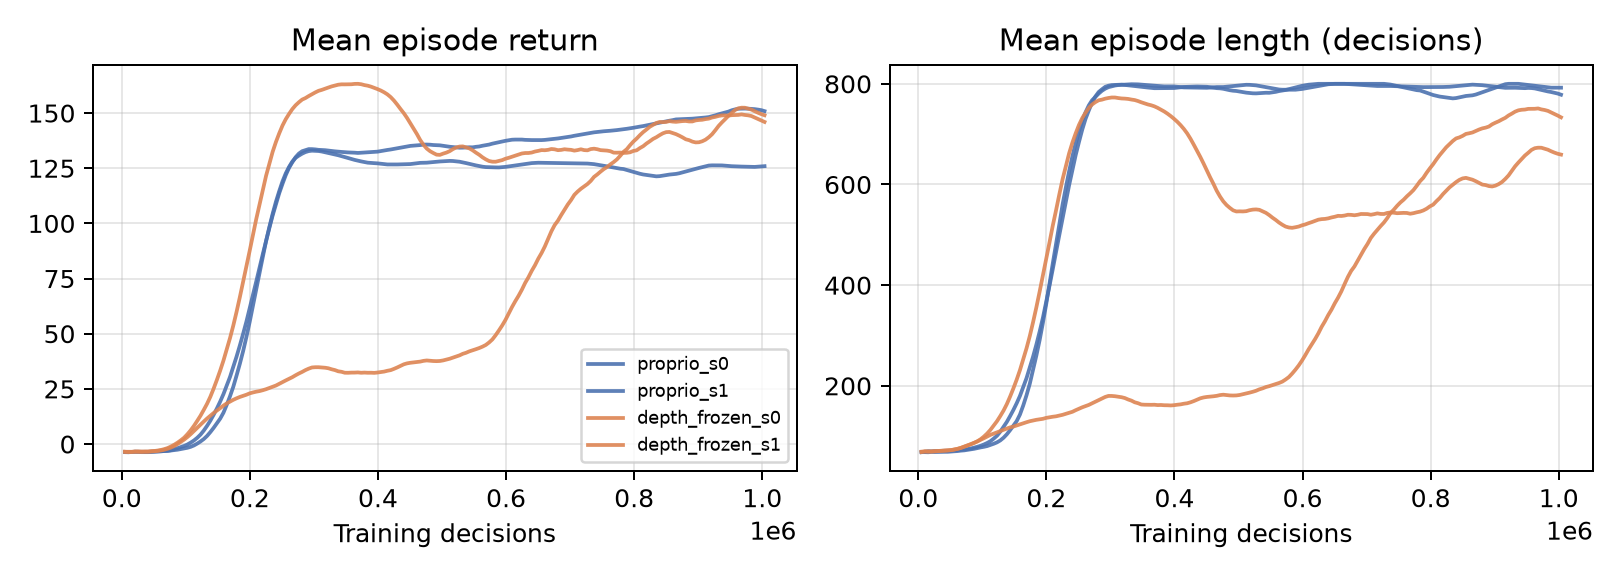
\includegraphics[width=\columnwidth]{figures/training_curves.png}
\caption{Training curves (mean over parallel environments). The drop in episode length after 0.5M decisions for some runs reflects episodes ending early on a fall or on reaching the 2\,m training goal.}\label{fig:train}
\end{figure}

\begin{table*}[t]
\centering\caption{H1: held-out terrains (clean depth). Success and fall rates in \% with 95\% Wilson intervals; pooled over training seeds. Time-to-goal is the mean over successful episodes.}\label{tab:h1}
\small\begin{tabular}{clcccrc}\toprule
Amplitude & Policy & $n$ & Success [\%] & Fall [\%] & Return & TTG [s]\\\midrule
0.04 & Prop.+depth & 60 & 100 [94, 100] & 0 [0, 6] & 168.4 & 4.6 \\
0.04 & Proprio & 60 & 55 [42, 67] & 0 [0, 6] & 145.0 & 5.3 \\
0.08 & Prop.+depth & 60 & 100 [94, 100] & 0 [0, 6] & 166.7 & 4.7 \\
0.08 & Proprio & 60 & 60 [47, 71] & 0 [0, 6] & 142.2 & 5.7 \\
0.12 & Prop.+depth & 60 & 88 [78, 94] & 12 [6, 22] & 153.0 & 4.9 \\
0.12 & Proprio & 60 & 57 [44, 68] & 8 [4, 18] & 126.5 & 6.0 \\
0.18 & Prop.+depth & 60 & 23 [14, 35] & 68 [56, 79] & 81.4 & 5.4 \\
0.18 & Proprio & 60 & 33 [23, 46] & 27 [17, 39] & 103.5 & 6.7 \\
\bottomrule\end{tabular}\end{table*}


\begin{figure}[t]
\centering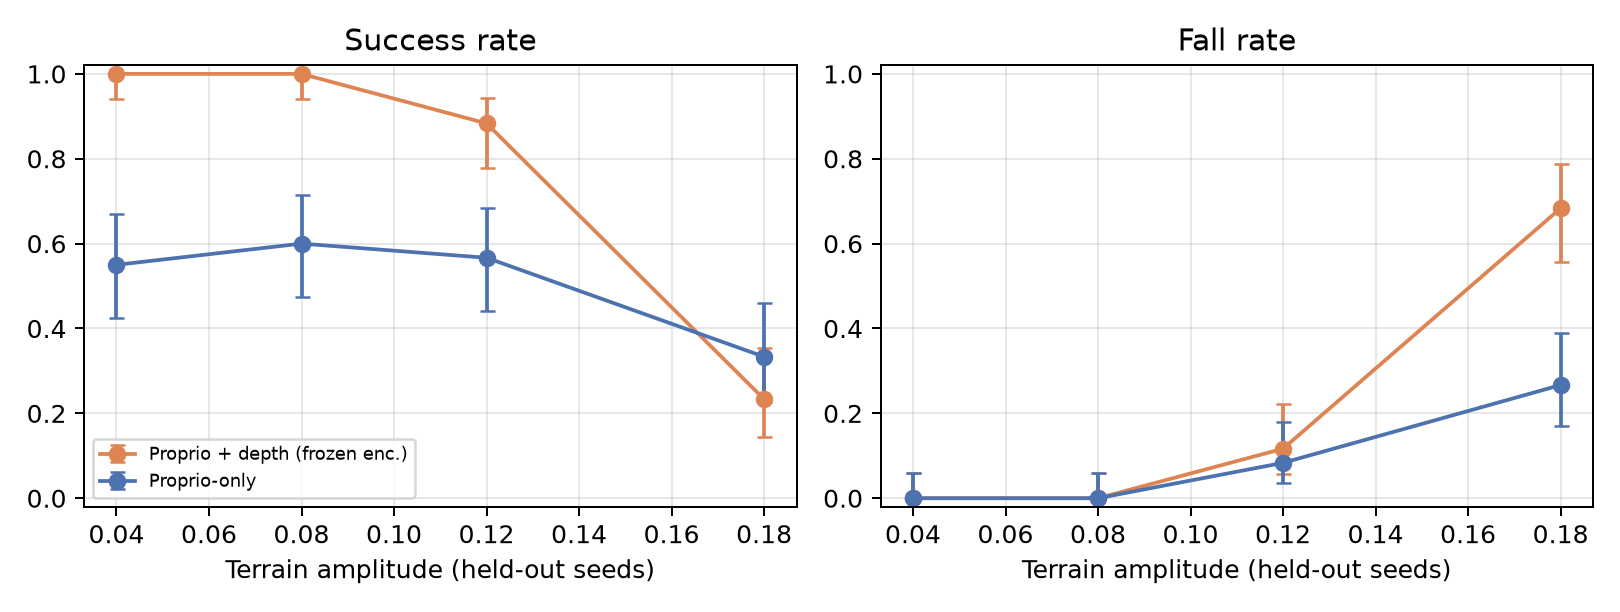
\includegraphics[width=\columnwidth]{figures/h1_success_fall.png}
\caption{H1: success and fall rate versus terrain amplitude (95\% Wilson intervals, pooled over two training seeds).}\label{fig:h1}
\end{figure}

\textbf{Result.} Pooled over the held-out terrains, the proprioception$+$depth policies reach the 1\,m goal more often than proprioception-only (paired difference $+0.27$, 95\% CI $[0.20,0.33]$, Wilcoxon $p<0.001$; Table~\ref{tab:tests}), but they also fall \emph{more} often ($+0.11$, CI $[0.06,0.17]$), mainly on the steepest terrain ($A{=}0.18$: 68\% vs.\ 27\% falls). The per-run breakdown shows that the pooled success gain is driven by a single slow policy: proprioception-only seed~0 succeeds on 85\% of episodes (depth seeds: 80\% and 76\%), whereas proprioception-only seed~1 learned a much slower gait (0.11\,m/s) and succeeds on only 18\%. Per-run mean falls are 11\%/7\% (proprio) vs.\ 16\%/24\% (depth). Hence H1 is \textbf{not supported}: with equal training budget, adding the frozen depth features did not reduce falls and did not give a reliable success benefit; the two-seed pooled test is dominated by seed variance and should be read as such.

\begin{table*}[t]
\centering\caption{Paired comparisons over identical held-out terrains (mean difference, bootstrap 95\% CI, Wilcoxon signed-rank $p$).}\label{tab:tests}
\scriptsize\begin{tabular}{lcccc}\toprule
Test & $n$ & $\Delta$ & 95\% CI & $p$\\\midrule
H1 success: depth frozen - proprio & 120 & +0.267 & [+0.196, +0.329] & <0.001 \\
H1 fell: depth frozen - proprio & 120 & +0.113 & [+0.058, +0.167] & <0.001 \\
H1 return: depth frozen - proprio & 120 & +13.107 & [+6.848, +19.295] & <0.001 \\
H2 success: depth frozen blank - clean & 60 & +0.008 & [-0.017, +0.042] & 0.564 \\
H2 success: depth frozen dropout 0.2 - clean & 60 & +0.008 & [+0.000, +0.025] & 0.317 \\
H2 success: depth frozen noise 0.05 - clean & 60 & +0.000 & [+0.000, +0.000] & 1.000 \\
H2 success: depth frozen noise 0.15 - clean & 60 & +0.000 & [+0.000, +0.000] & 1.000 \\
H2 success: depth frozen noise 0.30 - clean & 60 & +0.008 & [+0.000, +0.025] & 0.317 \\
H2 success: depth frozen occlusion 0.25 - clean & 60 & +0.000 & [+0.000, +0.000] & 1.000 \\
H2 success: depth frozen occlusion 0.50 - clean & 60 & +0.008 & [+0.000, +0.025] & 0.317 \\
H3 success: goal direction - goal relative & 90 & +0.000 & [+0.000, +0.000] & 1.000 \\
\bottomrule\end{tabular}\end{table*}



\subsection{H2: robustness to depth noise and occlusion}
We corrupt the depth channel at test time for both depth policies (3 amplitudes, 20 held-out terrains each; Table~\ref{tab:h2}, Fig.~\ref{fig:h2}). Corruptions: Gaussian noise ($\sigma_n=0.05,0.15,0.30$ in normalised depth, i.e.\ up to 30\,cm), 20\% pixel dropout, a square occluder covering 25\% or 50\% of each image, and a ``blank'' control where every pixel is invalid.

\begin{table*}[t]
\centering\caption{H2: depth corruption at test time (all amplitudes pooled).}\label{tab:h2}
\small\begin{tabular}{llcccc}\toprule
Policy & Condition & $n$ & Success [\%] & Fall [\%] & Return\\\midrule
Prop.+depth & blank & 120 & 70 & 28 & 131.3 \\
Prop.+depth & clean & 120 & 69 & 28 & 131.3 \\
Prop.+depth & dropout 0.2 & 120 & 70 & 28 & 131.3 \\
Prop.+depth & noise 0.05 & 120 & 69 & 28 & 131.3 \\
Prop.+depth & noise 0.15 & 120 & 69 & 28 & 131.3 \\
Prop.+depth & noise 0.30 & 120 & 70 & 28 & 131.3 \\
Prop.+depth & occlusion 0.25 & 120 & 69 & 28 & 131.3 \\
Prop.+depth & occlusion 0.50 & 120 & 70 & 28 & 131.3 \\
\bottomrule\end{tabular}\end{table*}


\begin{figure}[t]
\centering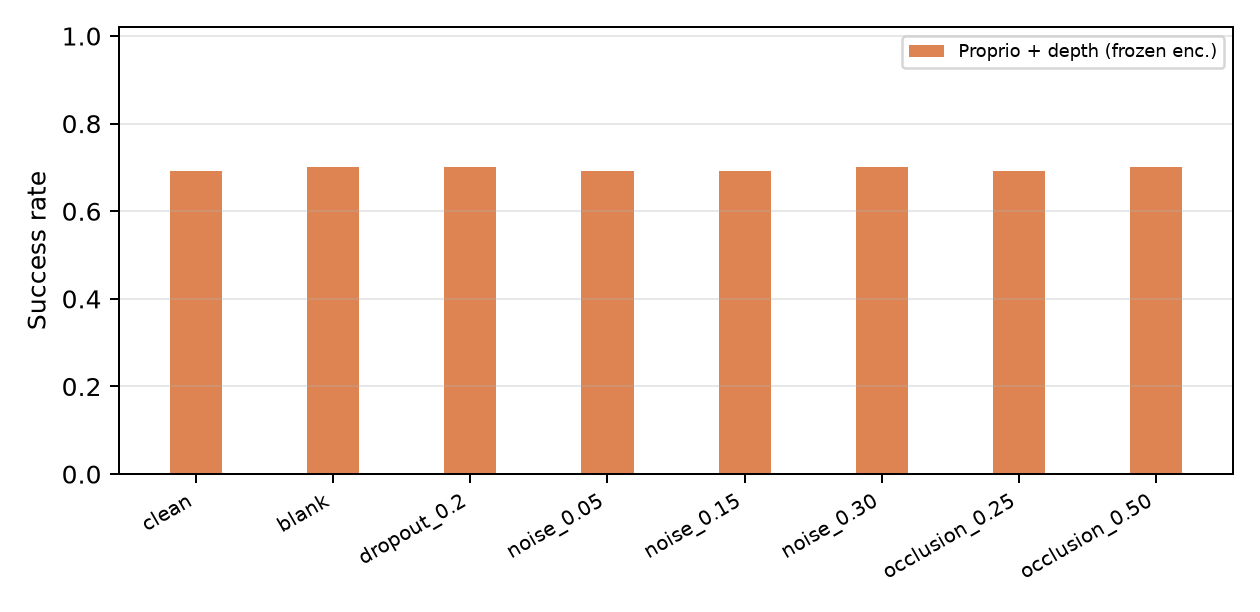
\includegraphics[width=\columnwidth]{figures/h2_robustness.png}
\caption{H2: success under depth corruption (depth policies; dashed line: proprio-only, clean).}\label{fig:h2}
\end{figure}

\textbf{Result.} Success and fall rates are unchanged by every corruption (all paired differences from the clean condition are within $\pm0.01$, $p\ge0.32$; Table~\ref{tab:tests}), \emph{including the blank-depth control}. We verified that the corruption does reach the policy (a $\sigma_n{=}0.3$ perturbation changes the observed image by 0.18 on average; the blank condition sets every pixel to 1). H2's premise, that performance drops when vision is degraded, is therefore \textbf{not observed}, and the reason is informative: the trained policies do not use the depth features. The $+$depth policies behave like proprioception-only policies with extra, ignored inputs, which is consistent with the H1 result. Plausible causes are that the terrains in the training range are shallow enough for proprioceptive feedback to suffice, that the frozen encoder was pretrained on a different terrain distribution, and the short training budget; these are tested in the next steps (Sec.~\ref{sec:concl}).


\subsection{H3 (stretch): goal-conditioned navigation}
We trained two proprioception-only policies with the same budget (1M decisions, one seed) on a waypoint task: a goal 2--3\,m away at a random bearing within $\pm60^\circ$ of the $+y$ axis, success when within 0.3\,m. The \emph{closed-loop} policy observes the goal position relative to the robot (2-d); the \emph{open-loop directional} policy observes only the unit direction to the goal at the start of the episode (no position feedback, no distance). Both are rewarded for speed toward the goal (the closed-loop one along the current bearing, the open-loop one along the initial bearing). We evaluate on 90 held-out terrains and goals each (amplitudes 0.04, 0.08, 0.12).

\textbf{Result (inconclusive; H3 not supported at this budget).} Neither policy reached the 0.3\,m goal radius within 8\,s (0/90 successes each), so time-to-goal cannot be compared. Using the reduction of goal distance instead, the open-loop directional policy was \emph{better}: it closed 51\% of the initial distance (mean final minimum distance 1.27\,m, 14\% of episodes within 0.6\,m) versus 30\% for the closed-loop policy (1.80\,m, 0\% within 0.6\,m); falls were 8\% and 2\%. This is the opposite of H3's prediction, but with speeds of roughly 0.1--0.2\,m/s a 2--3\,m goal is nearly out of reach in 8\,s, a single seed was trained, and the closed-loop reward changes direction as the robot moves, which slows credit assignment. We therefore report H3 as an unresolved stretch result and list the required follow-ups (longer episodes, goal-distance reward shaping, more seeds) in the next section.


%=====================================================================
\section{Conclusions and Next Steps}
%=====================================================================
\label{sec:concl}
\textbf{What we found.} (1) The released ballbot pipeline did not train on a stock simulator for three independent reasons (wrong friction frames on two of three wheels, a velocity-indexing bug that made the directional reward pay for angular velocity, and terrain 4--10$\times$ steeper than the tilt limit allows). After repairing them and re-tuning PPO (100\,Hz control, $\gamma{=}0.999$, a speed-capped reward and a fall penalty), policies learn to balance within $\approx$0.25M decisions and to drive at 0.1--0.2\,m/s on terrains of up to $\approx$9$^\circ$ mean slope, on held-out seeds. (2) \textbf{H1 is not supported}: frozen-encoder depth features did not lower the fall rate (they raised it on the steepest terrain) and gave no reliable success benefit once per-seed variation is considered. (3) \textbf{H2 is not observed} because the policies are insensitive even to fully blank depth, i.e.\ they ignore vision. (4) \textbf{H3 is inconclusive}: neither waypoint policy reached the goal in 8\,s.

\textbf{Limitations.} Two training seeds per variant (the pooled tests treat terrains as units and are dominated by seed variance); a 1M-decision budget, about one eighth of the baseline's 8M steps; a single frozen encoder pretrained on a different terrain distribution; success defined as 1\,m of progress because the policies are slow; one waypoint run; simulation only. The Python contact-frame fix reproduces the published patch's intent, not its exact numerical behaviour, and the NumPy gradient-noise fallback changes the exact terrains. Our absolute returns are not comparable to \cite{salehi2025} (different control rate and reward weights).

\textbf{Next steps.} (a) Make depth useful: train the encoder end-to-end or fine-tune it on this terrain distribution (\texttt{depth\_e2e} is implemented), add terrain types with features that cannot be felt before contact (steps, ridges), and use a harder curriculum so that proprioception alone is insufficient. (b) More seeds ($\ge5$) and a longer budget, with checkpoint selection on held-out terrains. (c) Re-run H3 with longer episodes and distance-based reward shaping. (d) Richer sensors and planning: a learned or map-based waypoint planner on top of the low-level policy (hierarchical control), and sim-to-real considerations such as domain randomisation.


\begin{thebibliography}{99}\small
\bibitem{salehi2025} A.~Salehi, ``Reinforcement learning for ballbot navigation in uneven terrain,'' arXiv:2505.18417, 2025.
\bibitem{salehi2025code} A.~Salehi, ``OpenBallBot-RL,'' \url{https://github.com/salehiac/OpenBallBot-RL}.
\bibitem{lauwers2006} T.~B.~Lauwers, G.~A.~Kantor, and R.~L.~Hollis, ``A dynamically stable single-wheeled mobile robot with inverse mouse-ball drive,'' in \emph{Proc.\ IEEE ICRA}, 2006, pp.~2884--2889.
\bibitem{nagarajan2014} U.~Nagarajan, G.~Kantor, and R.~Hollis, ``The ballbot: An omnidirectional balancing mobile robot,'' \emph{Int.\ J.\ Robotics Research}, vol.~33, no.~6, pp.~917--930, 2014.
\bibitem{schulman2017} J.~Schulman, F.~Wolski, P.~Dhariwal, A.~Radford, and O.~Klimov, ``Proximal policy optimization algorithms,'' arXiv:1707.06347, 2017.
\bibitem{schulman2016} J.~Schulman, P.~Moritz, S.~Levine, M.~Jordan, and P.~Abbeel, ``High-dimensional continuous control using generalized advantage estimation,'' in \emph{Proc.\ ICLR}, 2016.
\bibitem{todorov2012} E.~Todorov, T.~Erez, and Y.~Tassa, ``MuJoCo: A physics engine for model-based control,'' in \emph{Proc.\ IEEE/RSJ IROS}, 2012, pp.~5026--5033.
\bibitem{raffin2021} A.~Raffin \emph{et al.}, ``Stable-Baselines3: Reliable reinforcement learning implementations,'' \emph{J.\ Mach.\ Learn.\ Res.}, vol.~22, no.~268, pp.~1--8, 2021.
\bibitem{zhou2022} Y.~Zhou, J.~Lin, S.~Wang, and C.~Zhang, ``Learning ball-balancing robot through deep reinforcement learning,'' arXiv:2208.10142, 2022.
\bibitem{xiao2023} C.~Xiao \emph{et al.}, ``Design and control of a ballbot drivetrain with high agility, minimal footprint, and high payload,'' arXiv:2304.02887, 2023.
\bibitem{abdelrahim2025} M.~Abdelrahim \emph{et al.}, ``Modeling and control of a ballbot: A systematic approach,'' \emph{IEEE Access}, 2025, doi:10.1109/ACCESS.2025.3597797.
\bibitem{mavrogiannis2021} C.~Mavrogiannis, K.~Balasubramanian, S.~Poddar, A.~Gandra, and S.~S.~Srinivasa, ``Topology-informed model predictive control for anticipatory collision avoidance on a ballbot,'' 2021.
\bibitem{carius2022} J.~Carius, R.~Ranftl, F.~Farshidian, and M.~Hutter, ``Constrained stochastic optimal control with learned importance sampling: A path integral approach,'' \emph{Int.\ J.\ Robotics Research}, vol.~41, no.~2, 2022, doi:10.1177/02783649211047890.
\bibitem{hwangbo2019} J.~Hwangbo \emph{et al.}, ``Learning agile and dynamic motor skills for legged robots,'' \emph{Science Robotics}, vol.~4, no.~26, 2019.
\bibitem{lee2020} J.~Lee, J.~Hwangbo, L.~Wellhausen, V.~Koltun, and M.~Hutter, ``Learning quadrupedal locomotion over challenging terrain,'' \emph{Science Robotics}, vol.~5, no.~47, 2020.
\bibitem{miki2022} T.~Miki \emph{et al.}, ``Learning robust perceptive locomotion for quadrupedal robots in the wild,'' \emph{Science Robotics}, vol.~7, no.~62, 2022.
\bibitem{rudin2022} N.~Rudin, D.~Hoeller, P.~Reist, and M.~Hutter, ``Learning to walk in minutes using massively parallel deep reinforcement learning,'' in \emph{Proc.\ CoRL}, 2022.
\bibitem{perlin1985} K.~Perlin, ``An image synthesizer,'' in \emph{Proc.\ ACM SIGGRAPH}, 1985, pp.~287--296.
\bibitem{henderson2018} P.~Henderson \emph{et al.}, ``Deep reinforcement learning that matters,'' in \emph{Proc.\ AAAI}, 2018.
\bibitem{agarwal2021} R.~Agarwal \emph{et al.}, ``Deep reinforcement learning at the edge of the statistical precipice,'' in \emph{Proc.\ NeurIPS}, 2021.
\end{thebibliography}
\end{document}
